\section{Real data example}
\label{sec:regression-sec6}

\begin{figure}
%\captionsetup{justification=centering, font=footnotesize}
\begin{center}
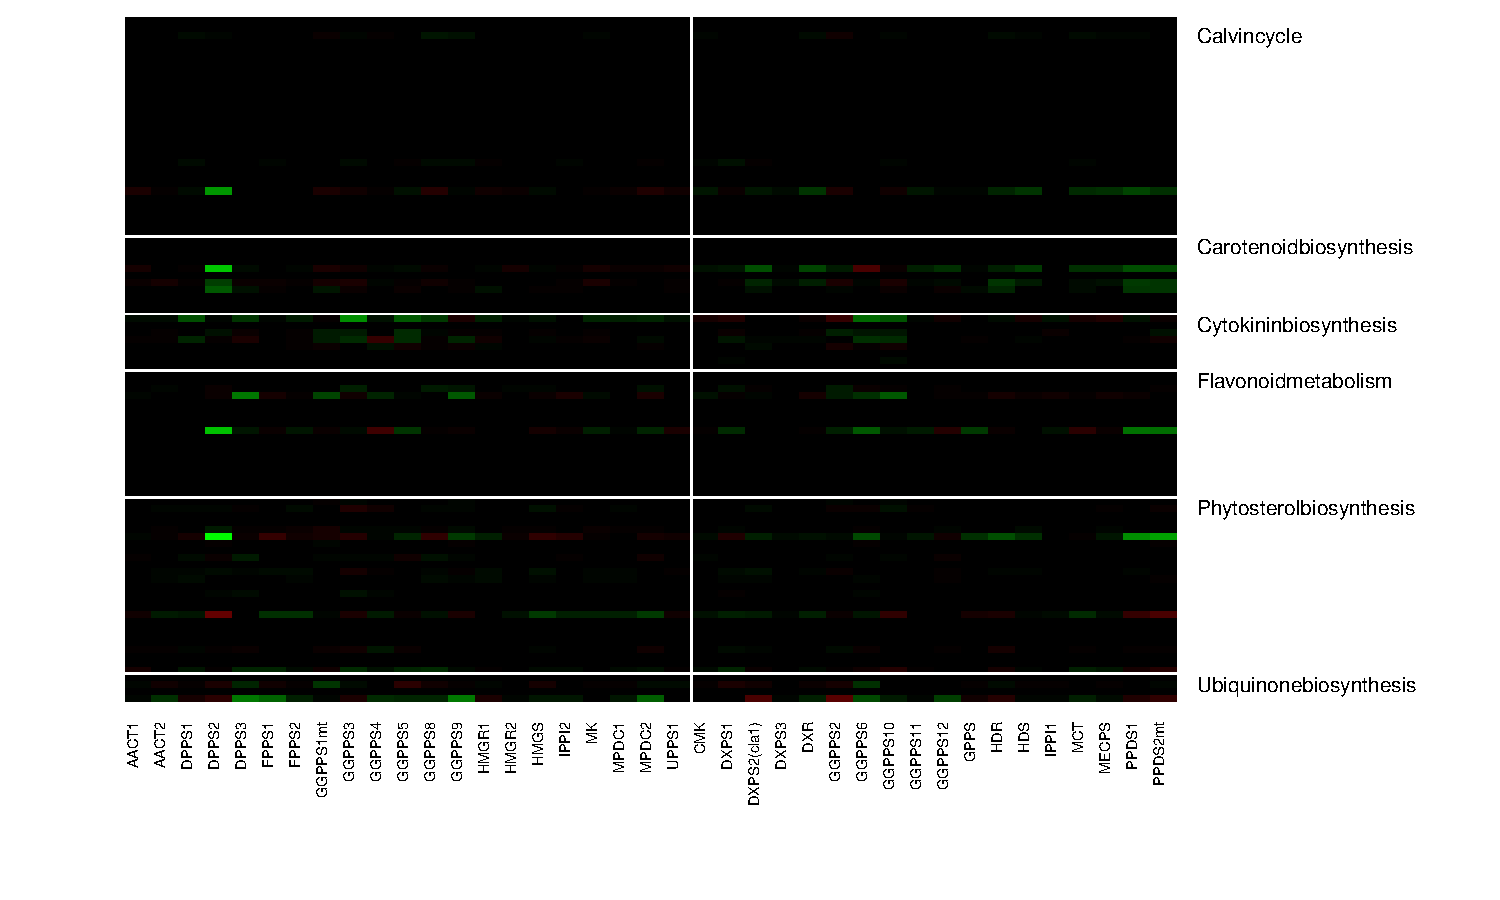
\includegraphics[width=.8\textwidth]{Chapter-regression/cropped_gene_heatmap1}

\caption{Estimated effects of different pathway genes on the activity of genes in Mevalonate and Non-mevalonate pathways (left and right of vertical line) in \textit{A. thaliana}}
\label{fig:coeffplots}
\end{center}
\end{figure}

\begin{table}[h]
\centering
\begin{footnotesize}
\begin{tabular}{rll}
  \hline
Coeff & Gene & Pathway \\ 
  \hline
0.18 & DPPS2 & Phytosterol biosynthesis \\ 
0.14 & DPPS2 & Carotenoid biosynthesis \\ 
0.14 & DPPS2 & Flavonoid metabolism \\ 
0.11 & DPPS2 & Calvin cycle \\ 
0.11 & PPDS2mt & Phytosterol biosynthesis \\ 
0.10 & GGPPS3 & Cytokinin biosynthesis \\ 
0.10 & PPDS1 & Phytosterol biosynthesis \\ 
0.09 & DPPS3 & Flavonoid metabolism \\ 
0.09 & DPPS3 & Ubiquinone biosynthesis \\ 
0.09 & GGPPS9 & Ubiquinone biosynthesis \\ 
\hline
\end{tabular}
\caption{Top 10 gene-pathway connections in {\it A. thaliana} data found by LARN}
\label{table:coefftable}
\end{footnotesize}
\end{table}

We apply the LARN algorithm on a microarray dataset containing expression of several genes in the flowering plant \textit{Arabidopsis thaliana} \citep{WilleEtal04}. In this dataset, gene expressions are collected from $n=118$ samples, which are plants grown under different experimental conditions. We take the expressions of $q=40$ genes in two pathways for biosynthesis of isoprenoid compounds, which are key compounds affecting plant metabolism as our multiple responses. Expressions of 795 other genes corresponding to 56 other pathways are taken as predictors.

Our objective here is to find out the extent of crosstalk between isoprenoid pathway genes and those in the other pathways. We apply LARN, as well as the two methods mentioned before, on the data and evaluate them based on predictive accuracy of 100 random splits with 90 training samples. All three methods have similar mean squared prediction error (MSPE) (LARN and GL-t have MSPE 0.45 and SGL has 0.44), but LARN produces more sparse solutions on average: the mean proportion of non-zero elements in the coefficient matrix are 0.15, 0.21 and 0.29 for LARN, GL-t and SGL, respectively. Focusing on the coefficient matrix estimated by LARN, we summarize the 10 largest coefficients (in absolute values) in \ref{table:coefftable}. We also visualize coefficients corresponding to genes in the 6 pathways in the table through a heatmap in  \ref{fig:coeffplots}.

All of the four largest coefficients correspond to interactions of one gene, DPPS2, with four different pathways. Two of these pathways, Carotenoid and Phytosterol, directly use products from the isoprenoid pathways, and their connections with DPPS2 had been detected in \cite{WilleEtal04}. The large Calvin Cycle-DPPS2 coefficient reveals that compounds synthesized in Carotenoid and Phytosterol pathways get used in Calvin Cycle. 
In the heatmap, Carotenoid biosynthesis seems to be connected mostly to the non-mevalonate pathway genes (right of the vertical line), while the activities of genes in Cytokinin and Ubiquinone synthesis pathways seem to be connected with those in the mevalonate pathway. These are consistent with the findings of \cite{WilleEtal04}, \cite{FrebortEtal11} and \cite{Disch98}, respectively.

\section{Conclusion}

In this chapter we propose a class of nonconvex penalty functions, based on the idea of inverting data depths, for performing support union recovery in multitask linear regression. Although several nonconvex penalties exist in the literature, the strength of our penalization scheme lies in the significant scope of inference procedures that can rise from the choice of the reference distribution $F$. Here we consider a simplified reference distribution and provide asymptotic oracle results that ensure recovery of the non-zero row support in the coefficient matrix. We also show that a simple post-estimation thresholding recovers non-zero elements within non-zero rows of the estimated coefficient matrix with good accuracy. Although our method shares the weakness of all nonconvex penalties: small signals may go undetected or can be estimated in a biased fashion, the flexibility in choosing $F$ provides enough motivation to fine tune similar penalization schemes. Our immediate plans for future studies include extending this specific setup to generalized linear models, dimensional asymptotics assuming the data dimension $p$ to be a function of sample size $n$, as well as exploring the use of more efficient algorithms for calculating the sparse solutions, e.g. proximal gradient descent or Concave-Convex algorithms \citep{WangKimLi13}.
